\documentclass[conference]{IEEEtran}
\IEEEoverridecommandlockouts

\usepackage{cite}
\usepackage{amsmath,amssymb,amsfonts}
\usepackage{algorithm}
\usepackage{algorithmic}
\usepackage{graphicx}
\usepackage{textcomp}
\usepackage{xcolor}
\usepackage{booktabs}
\usepackage{multirow}
\usepackage{url}

\graphicspath{{./}{../../experiments/paper_run_gpu_decision_cost/paper_assets/}{../../experiments/paper_run_final/paper_assets/}}

\newcommand{\MeanRho}{0.193}
\newcommand{\MedianRho}{0.180}
\newcommand{\MaxRho}{0.352}
\newcommand{\BeneficialCount}{8}
\newcommand{\DefaultSaferCount}{31}
\newcommand{\RunCount}{117}
\newcommand{\CaseCount}{13}
\newcommand{\SpeedupRange}{0.92--1.74$\times$}
\newcommand{\PredictionMAE}{47.5\%}
\newcommand{\ParallelPredictionMAE}{51.4\%}

\begin{document}

\title{Decision-Aware Execution Selection for Media Preprocessing}

\author{
\IEEEauthorblockN{First Author}
\IEEEauthorblockA{\textit{Department / Affiliation}\\
\textit{Institution}\\
City, Country\\
email@example.com}
\and
\IEEEauthorblockN{Second Author}
\IEEEauthorblockA{\textit{Department / Affiliation}\\
\textit{Institution}\\
City, Country\\
email@example.com}
\and
\IEEEauthorblockN{Third Author}
\IEEEauthorblockA{\textit{Department / Affiliation}\\
\textit{Institution}\\
City, Country\\
email@example.com}
}

\maketitle

\begin{abstract}
Media preprocessing is a common upstream stage in cloud and AI video pipelines, but the decision to parallelize such jobs is not free.
Short, content-variable clips may spend a meaningful fraction of their wall-clock time in metadata probing, feature extraction, scheduler search, chunk dispatch, and merge operations before or around the actual FFmpeg work.
This paper presents decision-aware execution selection for media preprocessing: a selector that models both execution overhead and decision overhead before choosing serial execution or a parallel worker/chunk plan.
We define $\rho = T_{\mathrm{decide}} / T_{\mathrm{execute}}$, where $T_{\mathrm{decide}}$ includes metadata probing, feature extraction, and scheduler search, and use it to characterize when adaptive selection is justified.
The implementation extracts lightweight video features, evaluates serial and parallel candidates with an overhead-aware cost model, and executes the selected FFmpeg plan using an automatically detected NVENC backend when available.
We evaluate \RunCount{} runs across \CaseCount{} video/workload cases with three preprocessing intensities and three baselines: serial, static equal-duration parallelism, and adaptive scheduling.
On the NVENC backend, adaptive selection is beneficial in only \BeneficialCount{} of 39 adaptive trials while the best non-adaptive default is safer in \DefaultSaferCount{} trials.
The mean decision-cost ratio is \MeanRho{} (median \MedianRho{}, maximum \MaxRho{}), and the selector's speedup over serial ranges from \SpeedupRange{}.
The GPU-backed results show that a CPU-calibrated selector does not automatically transfer to accelerated execution: prediction error rises to \PredictionMAE{} overall.
This negative result supports the paper's central claim: adaptive execution selection must include decision cost and must be calibrated on the target backend.
\end{abstract}

\begin{IEEEkeywords}
media preprocessing, execution selection, decision overhead, FFmpeg, NVENC, runtime modeling, cloud AI systems
\end{IEEEkeywords}

\section{Introduction}

Cloud video pipelines often preprocess media before the data reaches downstream AI stages such as object detection, scene classification, action recognition, or multimodal embedding.
This preprocessing can include normalization, sharpening, denoising, resizing, and other FFmpeg filter chains.
The inputs are highly variable: a pipeline may receive a short social-media clip, a medium-length phone recording, or a longer high-resolution video.
The preprocessing workload is also variable: a light color adjustment and a heavy denoise-sharpen chain have very different compute profiles.

A common implementation choice is to run the preprocessing stage with a fixed number of workers and a fixed chunking policy.
That is simple, but it hides two different costs.
First, parallel execution has orchestration overhead: chunks must be created, dispatched, processed independently, and merged.
Second, adaptive selection also has decision overhead: the system must probe metadata, extract features, and search candidate plans before it can choose a strategy.
For long or heavy jobs, this decision cost can be small relative to execution time.
For short media jobs, however, the decision layer itself may be large enough to remove the expected benefit of adaptivity.

This paper reframes the problem as \emph{decision-aware execution selection}.
Instead of asking only whether parallel processing is faster, we ask whether it is worth spending time to choose an execution plan for this specific job.
The selector must account for the total cost of choosing and executing a plan, not merely the predicted runtime of the selected plan.
This is important for short media jobs because a theoretically better plan can still be worse if discovering that plan takes too long.

We implement this idea in a research prototype for FFmpeg-based media preprocessing.
The system extracts lightweight content features, evaluates serial and parallel candidates, and selects a plan that may be serial or parallel.
For parallel plans, it chooses worker count, chunk count, and partitioning policy.
The same selector can run with a CPU backend or with an automatically detected NVIDIA NVENC backend.
The algorithm is unchanged across backends; only the FFmpeg execution backend changes.
This allows the model to be recalibrated for the actual hardware used in deployment.

The contributions are:
\begin{itemize}
\item We introduce a decision-cost view of media preprocessing and define $\rho = T_{\mathrm{decide}} / T_{\mathrm{execute}}$ as a measurable quantity for deciding when adaptive execution selection is worthwhile.
\item We implement an execution selector that accounts for metadata probing, feature extraction, scheduler search, orchestration overhead, and FFmpeg execution time while choosing serial or parallel execution.
\item We support both CPU and automatically detected NVENC execution backends, while preserving the same selector logic and recording the resolved backend in every experiment.
\item We provide a reproducible evaluation pipeline that emits per-run decision-cost fields, summary tables, and a paper-ready $\rho$ figure.
\end{itemize}

\section{Background and Motivation}

\subsection{Media Preprocessing in AI Pipelines}

Media preprocessing is the stage that converts raw uploaded or captured video into a form more suitable for later computation.
In AI pipelines, the preprocessing stage can be lightweight, such as contrast or brightness normalization, or heavier, such as denoising followed by sharpening.
Although this stage is often treated as a utility step, it can consume significant time when videos are processed at scale.

The preprocessing stage differs from model inference scheduling in two ways.
First, the unit of work is often a complete media object rather than a stream of independent inference requests.
Second, the runtime contains process-level and media-level overheads: FFmpeg startup, chunk boundary creation, dispatch, and concat-based merging.
These costs can dominate when clips are short.

\subsection{Why Decision Cost Matters}

Adaptive systems commonly assume that the time spent choosing a plan is negligible compared to the time spent executing the plan.
That assumption is reasonable for long batch jobs, but it is risky for short video preprocessing.
If a 4-second preprocessing task spends hundreds of milliseconds or more probing metadata, extracting features, and searching configurations, the selector must justify its own cost.

We therefore separate the decision phase from the execution phase:
\begin{equation}
T_{\mathrm{decide}} = T_{\mathrm{metadata}} + T_{\mathrm{features}} + T_{\mathrm{scheduler}},
\label{eq:tdecide}
\end{equation}
where $T_{\mathrm{metadata}}$ is FFprobe/container analysis, $T_{\mathrm{features}}$ is lightweight video feature extraction, and $T_{\mathrm{scheduler}}$ is candidate evaluation and search.
The execution phase is:
\begin{equation}
T_{\mathrm{execute}} = T_{\mathrm{dispatch}} + T_{\mathrm{compute}} + T_{\mathrm{merge}}.
\label{eq:texecute}
\end{equation}
We then define:
\begin{equation}
\rho = \frac{T_{\mathrm{decide}}}{T_{\mathrm{execute}}}.
\label{eq:rho}
\end{equation}
A high value of $\rho$ means that the selector is spending a large fraction of the job time deciding.
The GPU benchmark in this paper uses this value to characterize how much of each adaptive run is spent deciding rather than executing.

\section{System Design}

\subsection{Overview}

The system follows the same high-level structure as the earlier overhead-aware prototype.
An input video and filter chain pass through metadata probing, feature extraction, candidate generation, cost-model scoring, execution, and evaluation.
The key change is that the decision phase is now explicitly timed and recorded.
This makes the paper's central claim measurable rather than rhetorical.

\begin{figure*}[t]
\centering
\includegraphics[width=0.88\textwidth]{figure0_architecture.png}
\caption{System architecture. The selector receives metadata and low-cost content features, searches serial and parallel candidates, and records both decision cost and execution cost.}
\label{fig:arch}
\end{figure*}

\subsection{Feature Extraction}

The system extracts lightweight features from a downsampled representation of the video.
It samples frames at low temporal and spatial resolution and computes motion, scene-change frequency, luma variance, texture proxy, bitrate, and bits-per-pixel statistics.
These features are not intended to replace the full preprocessing job.
They are a low-cost signal used to estimate the relative cost of candidate execution plans.

For segment $i$, the estimated complexity is:
\begin{equation}
\hat{C}_i = d_i \cdot r \cdot \phi \cdot
(0.45 + 0.25m_i + 0.15s_i + 0.10v_i + 0.05\tau_i) \cdot \beta_i,
\label{eq:complexity}
\end{equation}
where $d_i$ is segment duration, $r$ is a resolution factor, $\phi$ is a filter-chain weight, and $m_i$, $s_i$, $v_i$, $\tau_i$, and $\beta_i$ represent motion, scene change, variance, texture, and bitrate scaling.

\subsection{Candidate Plans}

The selector considers serial execution and parallel execution.
For parallel execution, it searches worker counts, chunk counts, and partitioning policies.
The partitioning policies are:
\begin{itemize}
\item \textbf{Equal-duration:} split the clip into chunks with equal time length.
\item \textbf{Rate-adjusted:} estimate serial encoding rate at several positions and place chunk boundaries by cumulative work.
\item \textbf{Cost-balanced:} use segment complexity estimates to create chunks with more balanced predicted costs.
\end{itemize}

The selected plan is executed by launching FFmpeg workers over the selected chunks and merging the outputs with the concat demuxer.
If stream-copy merge fails, the system falls back to a re-encoded merge.

\subsection{CPU and NVENC Backends}

The implementation supports three backend modes: \texttt{cpu}, \texttt{cuda}, and \texttt{auto}.
The \texttt{cpu} mode uses \texttt{libx264}.
The \texttt{cuda} mode uses \texttt{h264\_nvenc} for encoding.
The \texttt{auto} mode first checks whether FFmpeg can actually complete a small NVENC encode and uses NVENC only if that test succeeds.
Otherwise, it falls back to CPU execution.

This backend change does not alter the selector algorithm.
It changes the measured execution platform, which is why every run records the requested backend, resolved backend, and NVENC availability.
All reported results in this draft use one resolved backend policy: \texttt{auto} resolved to \texttt{cuda}, with NVENC available.

\section{Decision-Aware Selection}

\subsection{Cost Model}

For a serial candidate, the system estimates:
\begin{equation}
\hat{T}_s = d \cdot \max(0.2, r) \cdot \phi \cdot \mu,
\label{eq:serial}
\end{equation}
where $d$ is duration, $r$ is the resolution factor, $\phi$ is the filter-chain complexity weight, and $\mu$ is a motion-adjusted factor.

For a parallel candidate with $w$ workers, $c$ chunks, and estimated chunk costs $C = [\hat{C}_1, \ldots, \hat{C}_c]$, the predicted runtime is:
\begin{equation}
\hat{T}_p = \alpha(w,c,r) \cdot M(C,w) + T_{\mathrm{oh}}(w,c,d),
\label{eq:parallel}
\end{equation}
where $M(C,w)$ is the makespan estimated by greedy list scheduling and $T_{\mathrm{oh}}$ includes dispatch, merge, and startup overhead.

\subsection{Selection Rule}

The selector searches candidate parallel plans and compares the best predicted parallel runtime to the estimated serial runtime.
A serial gate prevents parallel execution when the predicted improvement is too small to survive overhead noise.
The decision-aware extension adds a second reporting layer: even if the selected plan is faster than a fixed default, we measure how much time was spent making that decision.
This does not require inventing a universal threshold for $\rho$.
Instead, the final results will empirically show the region where adaptive selection pays off and the region where a default strategy is safer.

\begin{algorithm}[t]
\caption{Decision-Aware Execution Selection}
\label{alg:select}
\begin{algorithmic}[1]
\REQUIRE input video $x$, filter chain $f$, worker budget $w_{\max}$
\ENSURE selected execution plan
\STATE Measure $T_{\mathrm{metadata}}$ while probing input metadata
\STATE Extract low-cost features and measure $T_{\mathrm{features}}$
\STATE Estimate serial runtime $\hat{T}_s$
\STATE Enumerate admissible parallel candidates $(w,c,p)$
\STATE Score candidates using Eq.~\ref{eq:parallel}
\STATE Measure scheduler search time $T_{\mathrm{scheduler}}$
\STATE Compute $T_{\mathrm{decide}}$ using Eq.~\ref{eq:tdecide}
\IF{best parallel candidate clears the serial safety margin}
\RETURN selected parallel plan
\ELSE
\RETURN serial plan
\ENDIF
\end{algorithmic}
\end{algorithm}

\section{Experimental Methodology}

\subsection{Workloads}

The benchmark uses three preprocessing intensities:
\begin{itemize}
\item \textbf{Light:} brightness, contrast, and saturation normalization.
\item \textbf{Medium:} unsharp masking for detail enhancement.
\item \textbf{Heavy:} denoise, blur, and sharpen chain for robust preprocessing.
\end{itemize}

The benchmark suite contains four main input videos evaluated under all three workloads, plus one short 3\,s light-workload case.
This produces \CaseCount{} video/workload cases and \RunCount{} total runs: three baselines, three trials per case.

\subsection{Baselines}

We compare:
\begin{itemize}
\item \textbf{Serial:} one FFmpeg process, no chunk-level parallelism.
\item \textbf{Static-equal:} fixed worker count and equal-duration chunking.
\item \textbf{Adaptive-scheduled:} the full decision-aware selector.
\end{itemize}

\subsection{Metrics}

The evaluation reports:
\begin{itemize}
\item Runtime and speedup versus serial.
\item Decision cost $T_{\mathrm{decide}}$.
\item Execution cost $T_{\mathrm{execute}}$.
\item Decision-cost ratio $\rho$.
\item Prediction error of the runtime model.
\item Output quality using PSNR and SSIM against the reference output.
\item Backend metadata showing whether the run used CPU or NVENC.
\end{itemize}

\subsection{Hardware}

Experiments were run on a GPU-capable laptop with an NVIDIA RTX 3060 GPU with 6 GB VRAM, 32 GB RAM, and FFmpeg NVENC acceleration enabled through WSL.
The selector logic was unchanged; only the FFmpeg execution backend changed from CPU x264 to NVENC where available.
The experiment manifest records \texttt{execution\_backend.requested=auto}, \texttt{execution\_backend.resolved=cuda}, and \texttt{nvenc\_available=true}.
The CPU model, FFmpeg version, driver version, and WSL version should be inserted before submission.

\section{Results}

\subsection{Decision-Cost Characterization}

The main result of the revised paper is the decision-cost analysis.
Fig.~\ref{fig:rho} plots $\rho$ against the best non-adaptive default runtime.
Green points indicate cases where adaptive selection beats the best default, and red points indicate cases where the default is safer.
Across 39 adaptive-scheduled trials, mean $\rho$ is \MeanRho{}, median $\rho$ is \MedianRho{}, and maximum $\rho$ is \MaxRho{}.
Adaptive selection is beneficial in \BeneficialCount{} trials, while the best non-adaptive default is safer in \DefaultSaferCount{} trials.
The mean adaptive-vs-default margin is $-6.9\%$, which means that the adaptive selector is slower than the best default on average under this NVENC-backed execution regime.

\begin{figure}[t]
\centering
\IfFileExists{figure5_decision_cost_rho.pdf}
{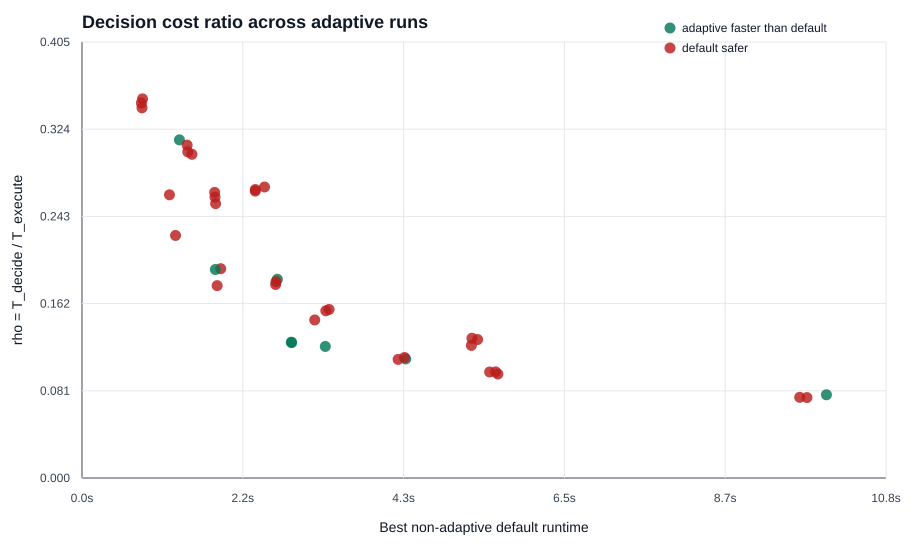
\includegraphics[width=\columnwidth]{figure5_decision_cost_rho.pdf}}
{\IfFileExists{figure5_decision_cost_rho.png}
{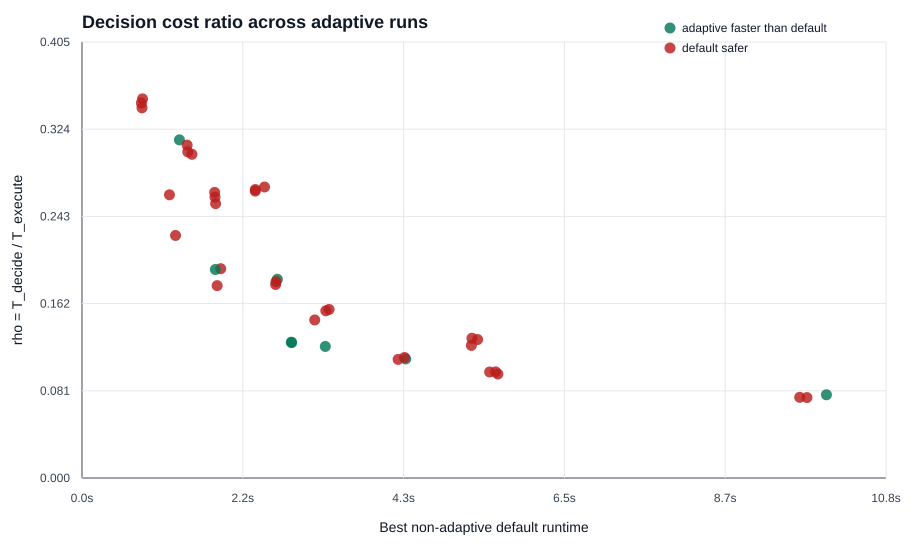
\includegraphics[width=\columnwidth]{figure5_decision_cost_rho.png}}
{\fbox{\parbox{0.92\columnwidth}{\centering Decision-cost rho figure unavailable to LaTeX until \texttt{figure5\_decision\_cost\_rho.svg} is exported as PDF or PNG. Table~\ref{tab:decision-cost} reports the same summary.}}}}
\caption{Decision-cost ratio $\rho = T_{\mathrm{decide}} / T_{\mathrm{execute}}$ across adaptive-scheduled runs. Green points indicate trials where adaptive selection beats the best non-adaptive default; red points indicate trials where the default is safer.}
\label{fig:rho}
\end{figure}

\begin{table}[t]
\caption{Decision-cost summary for adaptive-scheduled trials.}
\label{tab:decision-cost}
\centering
\begin{tabular}{lc}
\toprule
Metric & Value \\
\midrule
Adaptive trials & 39 \\
Mean $\rho$ & \MeanRho{} \\
Median $\rho$ & \MedianRho{} \\
Maximum $\rho$ & \MaxRho{} \\
Adaptive beneficial & \BeneficialCount{}/39 \\
Default safer & \DefaultSaferCount{}/39 \\
Mean adaptive margin vs.\ default & $-6.9\%$ \\
\bottomrule
\end{tabular}
\end{table}

\subsection{Runtime Performance}

Table~\ref{tab:runtime-summary} summarizes the case-level outcome.
Static equal-duration parallelism wins 10 of 13 cases, adaptive-scheduled wins 2 cases, and serial wins 1 case.
The selector makes a good decision in 8 of 13 cases, where good means that its execution is within 5\% of the winner or uses the same effective configuration.
The selector's speedup over serial ranges from \SpeedupRange{}, with a mean of 1.27$\times$.
These results differ from the earlier CPU-only behavior: under NVENC, fixed parallelism is often strong enough that the adaptive selector's extra decision path is not always justified.

\begin{figure*}[t]
\centering
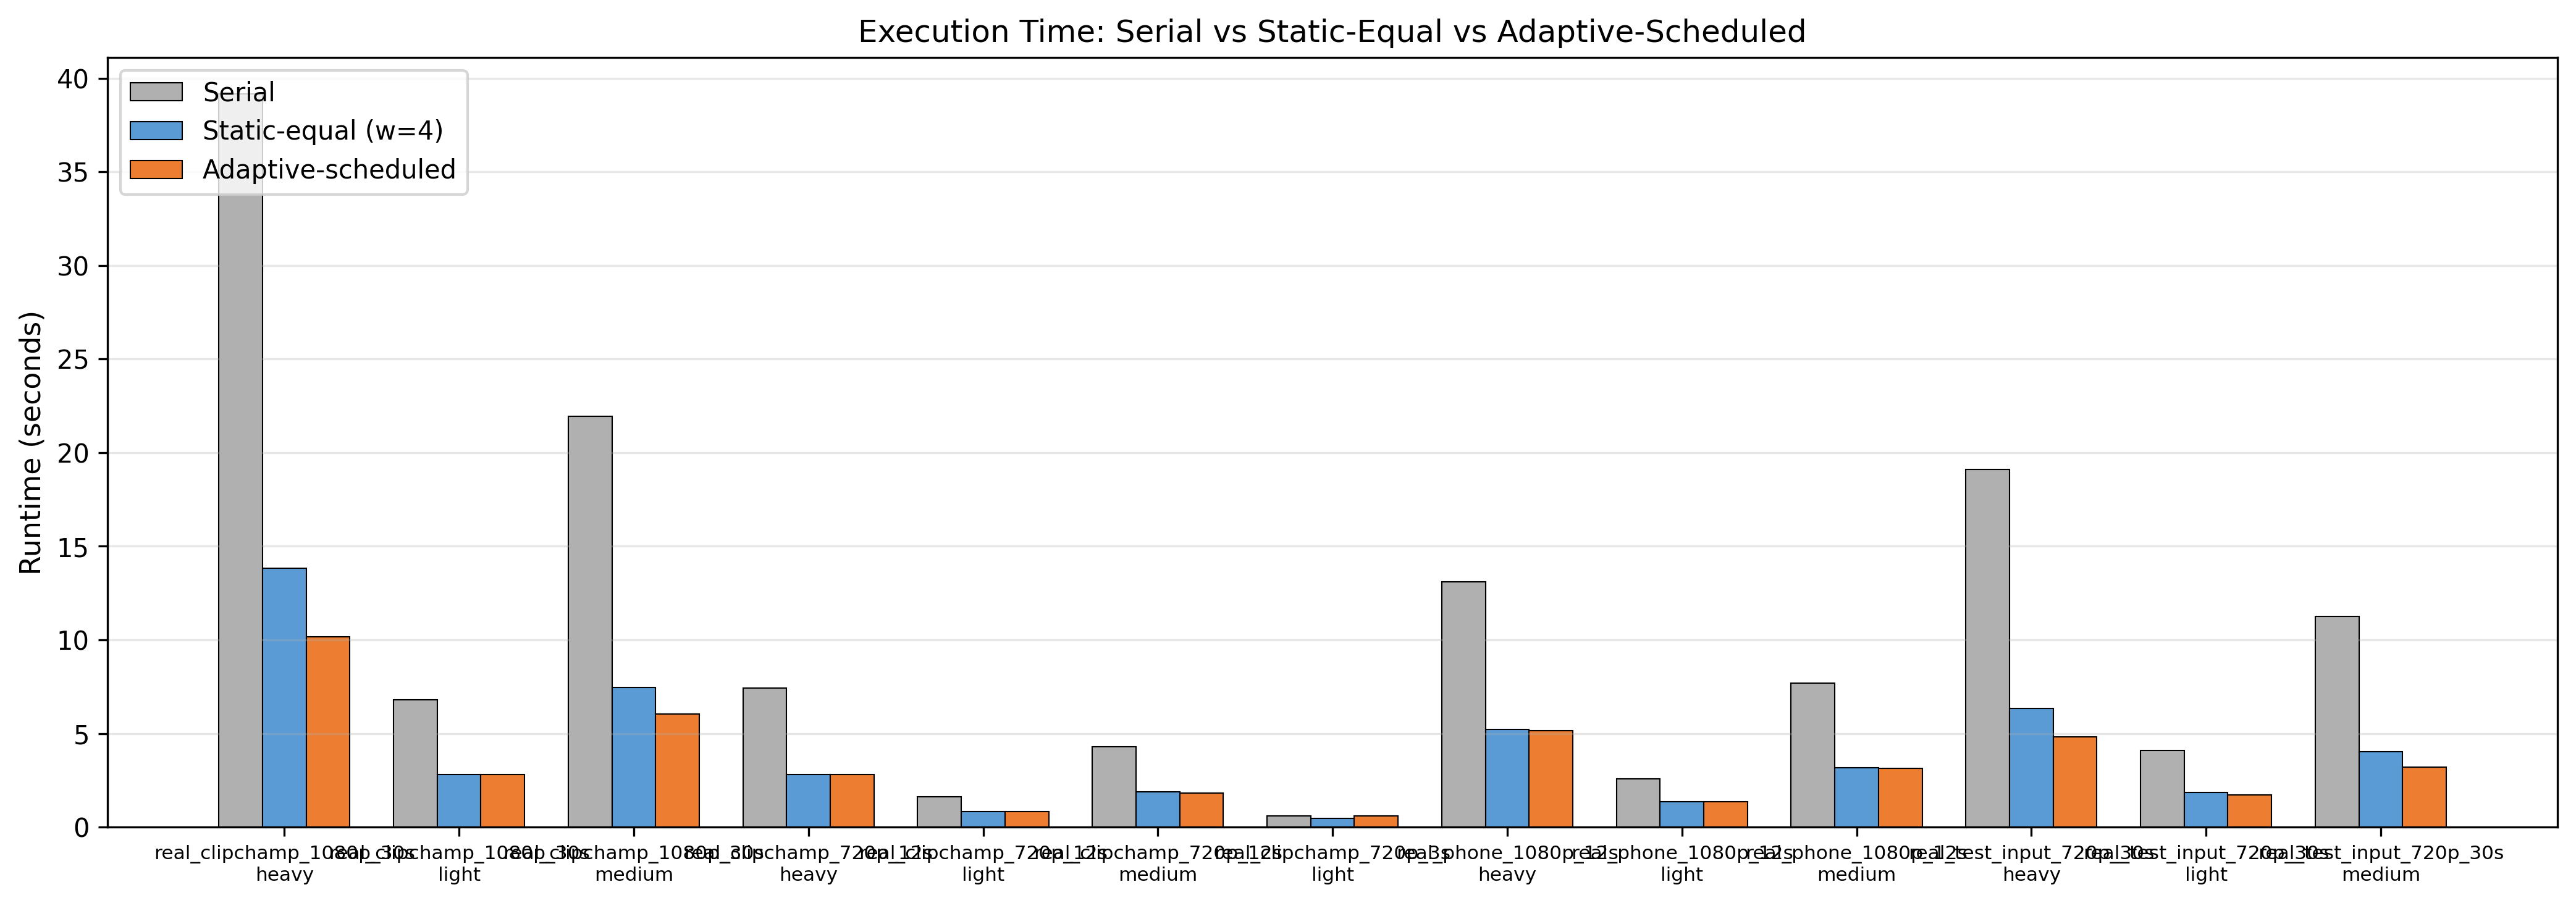
\includegraphics[width=\textwidth]{figure1_speedup_comparison.png}
\caption{Speedup comparison. This figure should be regenerated from the GPU run before final submission; Table~\ref{tab:runtime-summary} reports the current GPU-backed summary.}
\label{fig:speedup}
\end{figure*}

\begin{table}[t]
\caption{Case-level winner summary under NVENC-backed execution.}
\label{tab:runtime-summary}
\centering
\begin{tabular}{lc}
\toprule
Metric & Value \\
\midrule
Video/workload cases & \CaseCount{} \\
Total runs & \RunCount{} \\
Static-equal wins & 10/13 \\
Adaptive-scheduled wins & 2/13 \\
Serial wins & 1/13 \\
Good selector decisions & 8/13 \\
Selector speedup vs.\ serial & \SpeedupRange{} \\
Mean selector speedup vs.\ serial & 1.27$\times$ \\
\bottomrule
\end{tabular}
\end{table}

\subsection{Prediction Accuracy}

The generated calibration report shows that the existing cost model overfits the CPU execution regime and does not transfer cleanly to NVENC.
Overall prediction mean absolute error is \PredictionMAE{}, and parallel-only error is \ParallelPredictionMAE{}.
Error is 47.4\% for heavy workloads, 56.0\% for medium workloads, and 40.7\% for light workloads.
This is not a failure of the decision-cost framing; it is evidence for it.
When the execution backend changes, the runtime model must be recalibrated, and the selector must account for its own decision cost before it can be trusted.

\begin{figure}[t]
\centering
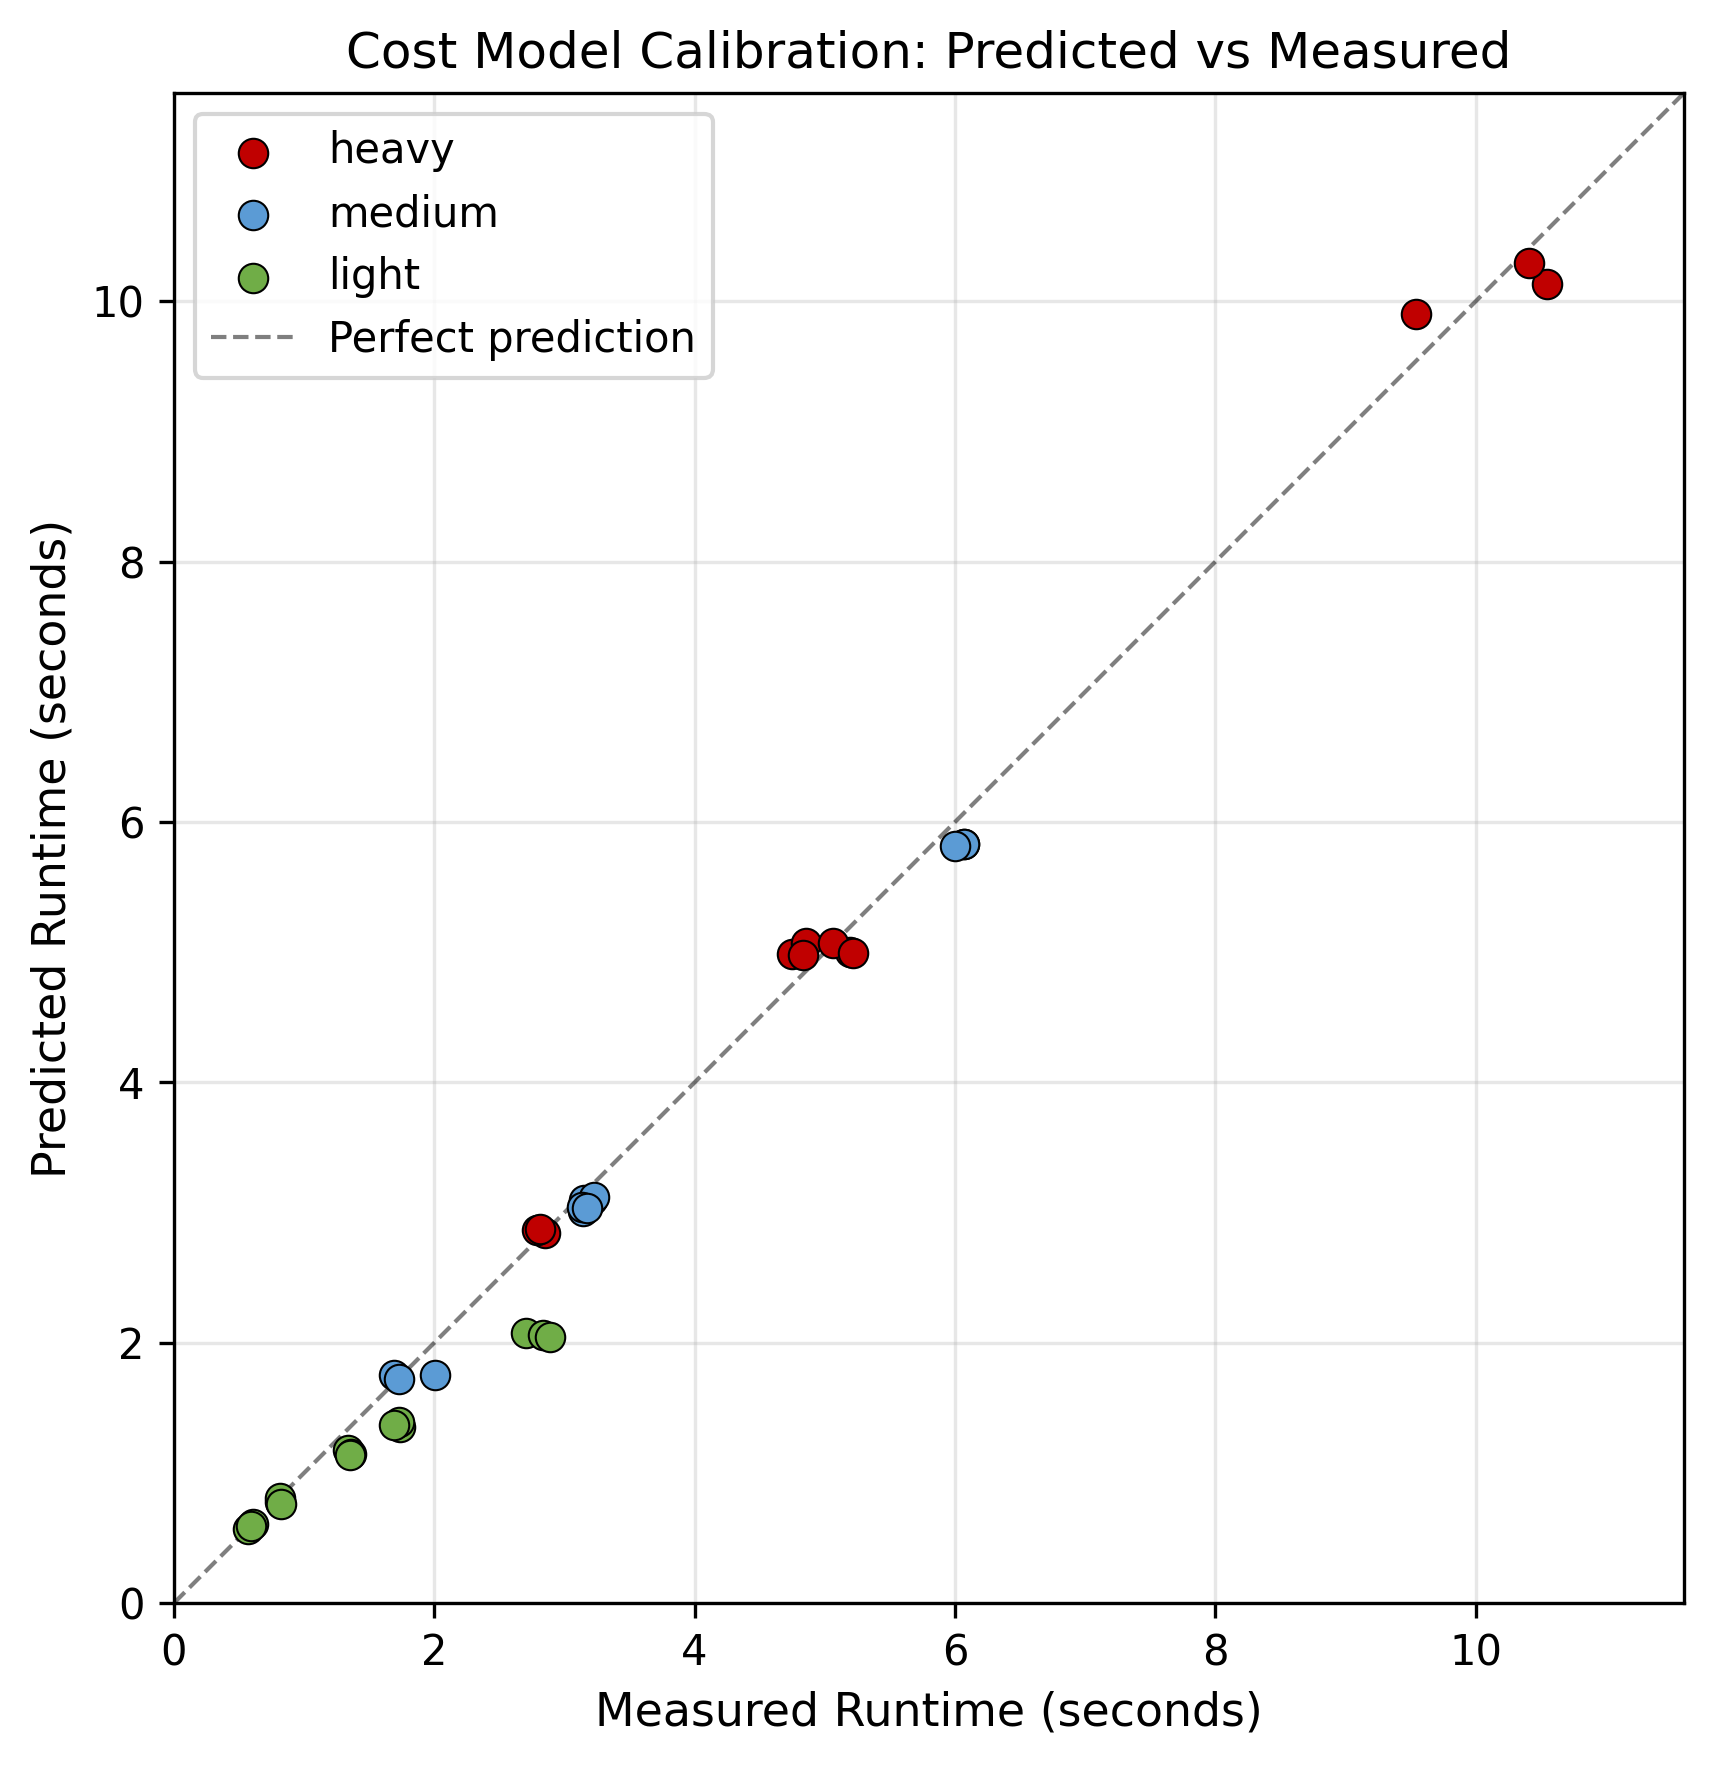
\includegraphics[width=\columnwidth]{figure2_calibration_scatter.png}
\caption{Predicted versus measured runtime. The GPU-backed run shows that the CPU-calibrated model substantially underpredicts NVENC-backed execution time.}
\label{fig:calibration}
\end{figure}

\subsection{Resource Budgets}

The selector can operate under a worker budget.
In the GPU-backed budget analysis, the selector chooses parallel execution in 12 of 13 cases for every budget setting ($w \le 2$, $w \le 4$, $w \le 8$, and unconstrained), and serial execution only for the 3\,s light case.
This stability across budgets indicates that, under NVENC, the selected regime is less sensitive to worker budget than it was in the CPU-oriented framing.
The more important distinction becomes whether adaptive selection is worth performing at all relative to a strong static default.

\begin{figure}[t]
\centering
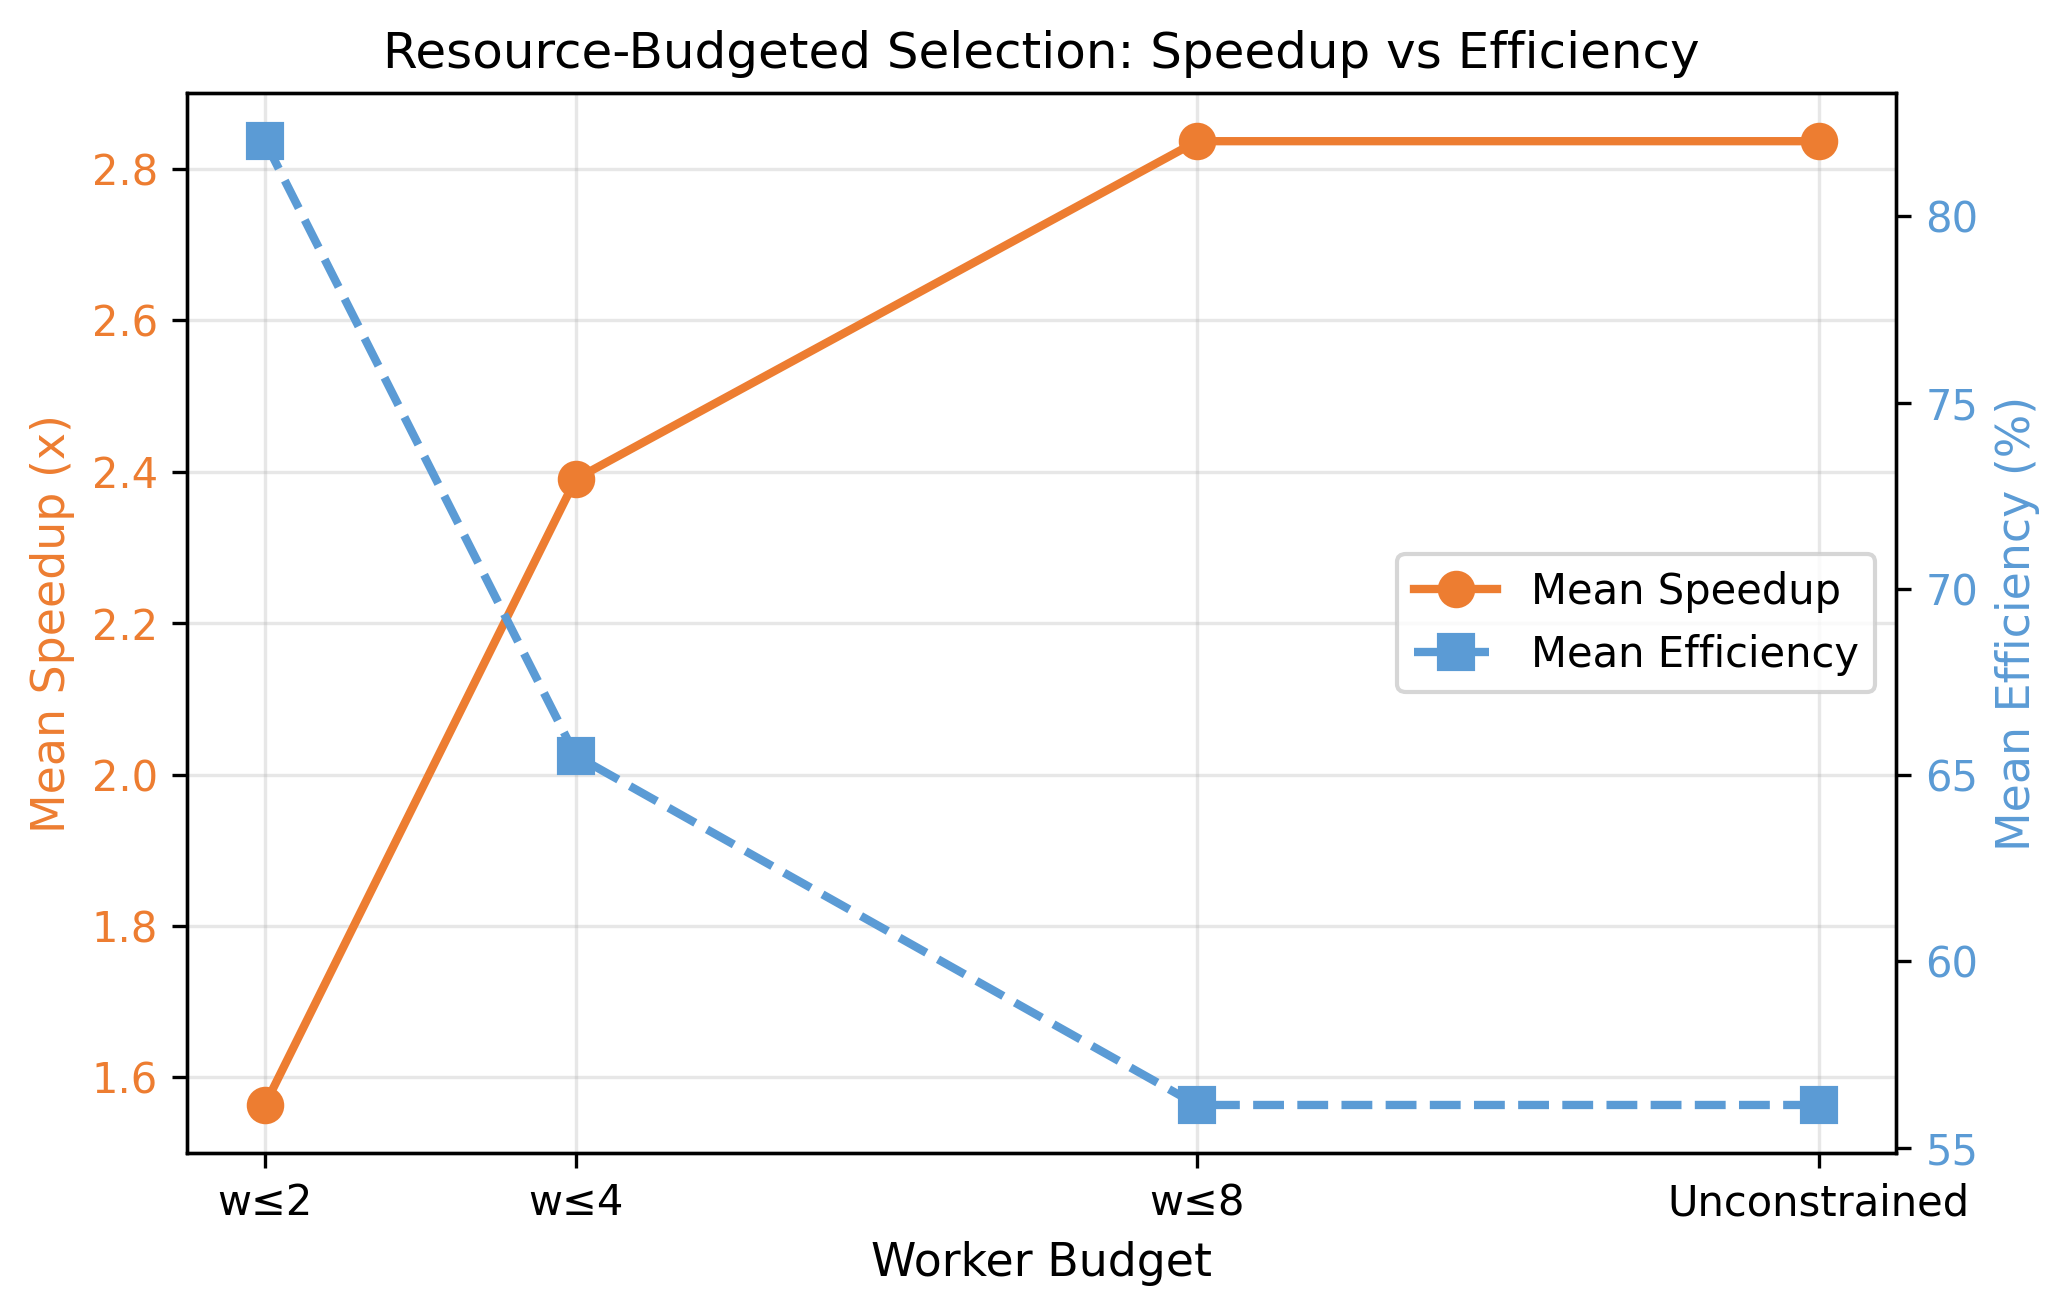
\includegraphics[width=\columnwidth]{figure3_budget_tradeoffs.png}
\caption{Worker-budget tradeoff. This figure should be regenerated from the GPU run before final submission.}
\label{fig:budget}
\end{figure}

\subsection{Output Quality}

For each processed output, the evaluator computes PSNR and SSIM against a reference output.
Across adaptive-scheduled runs, PSNR ranges from 23.68\,dB to 49.77\,dB with a mean of 36.03\,dB on runs where PSNR is defined.
SSIM ranges from 0.915 to 1.000 with a mean of 0.976.
The lowest values occur on heavier enhancement chains where the filter itself changes the signal more strongly, but the average SSIM indicates that chunk-parallel execution does not introduce severe structural degradation.

\section{Discussion}

\subsection{What the Decision-Cost View Adds}

The previous framing was mainly overhead-aware: it asked whether parallel execution is worth dispatch and merge overhead.
The revised framing is broader: it asks whether the decision procedure itself is worth paying for.
This is a more defensible contribution because it treats adaptive scheduling as a costed operation rather than assuming the selector is free.

\subsection{Why Hardware Backend Matters}

The value of adaptive selection depends on the execution platform.
On a CPU backend, FFmpeg compute may dominate for heavy filters, making parallelism attractive.
On an NVENC backend, the relative balance changes: fixed equal-duration parallelism wins 10 of 13 cases, and adaptive scheduling is beneficial in only \BeneficialCount{} of 39 adaptive trials.
This does not invalidate the selector.
Instead, it supports the paper's central claim: decision overhead and runtime prediction must be measured on the target backend.
An execution selector calibrated on CPU behavior should not be assumed to remain optimal after the encoder changes.

\subsection{Interpreting Short Jobs}

Short jobs are the critical regime.
They can be too small for parallel execution and too small for expensive selection.
The goal is not to force adaptivity everywhere.
The goal is to identify the regime in which adaptive selection is beneficial and the regime in which a default strategy is safer.

\section{Limitations and Threats to Validity}

\textbf{Single-machine evaluation.}
The final results are measured on one GPU-capable laptop.
The values of $T_{\mathrm{decide}}$, $T_{\mathrm{execute}}$, and $\rho$ may change on cloud VMs, multi-node systems, or different GPUs.

\textbf{Backend-specific coefficients.}
The selector logic is backend-independent, but the measured cost coefficients are not.
A CPU-calibrated model should not be assumed to generalize to NVENC without recalibration.

\textbf{Workload diversity.}
The benchmark includes representative FFmpeg preprocessing chains, but it does not cover every filter, codec, resolution, or live-stream condition.

\textbf{Decision threshold.}
This draft does not claim a universal $\rho$ threshold.
The threshold should be derived from the final benchmark data, if the data supports one.

\textbf{Reference integrity.}
All references and DOIs should be manually verified before submission.

\section{Conclusion}

This paper presents decision-aware execution selection for media preprocessing.
The main idea is simple: adaptive execution selection has a cost, and that cost must be measured alongside execution overhead.
By recording $T_{\mathrm{metadata}}$, $T_{\mathrm{features}}$, $T_{\mathrm{scheduler}}$, $T_{\mathrm{execute}}$, and $\rho$, the system can explain when adaptive selection is useful and when a default strategy is safer.

In \RunCount{} NVENC-backed runs, adaptive selection is beneficial in \BeneficialCount{} of 39 adaptive trials, while a non-adaptive default is safer in \DefaultSaferCount{} trials.
Mean $\rho$ is \MeanRho{} and reaches \MaxRho{}, showing that decision cost is a measurable fraction of execution time.
The contribution is not that GPU execution is faster, but that the decision-aware framework remains measurable and backend-specific: the selector must be evaluated and calibrated on the hardware where it will run.

\section*{Acknowledgment}
Acknowledgments or funding information can be added here.

\begin{thebibliography}{00}
\bibitem{amdahl1967} G. M. Amdahl, ``Validity of the single processor approach to achieving large scale computing capabilities,'' in \emph{Proc. AFIPS Spring Joint Computer Conference}, 1967, pp. 483--485.
\bibitem{graham1969} R. L. Graham, ``Bounds on multiprocessing timing anomalies,'' \emph{SIAM Journal on Applied Mathematics}, vol. 17, no. 2, pp. 416--429, 1969.
\bibitem{ffmpegdocs} FFmpeg Developers, ``FFmpeg documentation,'' \url{https://ffmpeg.org/documentation.html}.
\bibitem{jokhio2013} F. A. Jokhio, A. Ashraf, S. Lafond, I. Porres, and J. Lilius, ``Prediction-based dynamic resource allocation for video transcoding in cloud computing,'' in \emph{Proc. PDP}, 2013, pp. 254--261.
\bibitem{li2018} X. Li, M. A. Salehi, M. Bayoumi, N. Tzeng, and R. Buyya, ``Cost-efficient and robust on-demand video transcoding using heterogeneous cloud services,'' \emph{IEEE Transactions on Parallel and Distributed Systems}, vol. 29, no. 3, pp. 556--571, 2018.
\bibitem{kubernetes} Kubernetes Authors, ``Horizontal Pod Autoscaling,'' \url{https://kubernetes.io/docs/tasks/run-application/horizontal-pod-autoscale/}.
\end{thebibliography}

\end{document}
